\documentclass[conference]{IEEEtran}
\IEEEoverridecommandlockouts
% The preceding line is only needed to identify funding in the first footnote. If that is unneeded, please comment it out.
\usepackage{cite}
\usepackage{amsmath,amssymb,amsfonts}
\usepackage{algorithmic}
\usepackage{graphicx}
\usepackage{textcomp}
\usepackage{subcaption}
\usepackage[spanish]{babel}
\usepackage{hyperref}
\usepackage{array}
\usepackage{listings}
\usepackage{float}
\usepackage{xcolor}
\definecolor{codegreen}{rgb}{0,0.6,0}
\definecolor{codegray}{rgb}{0.5,0.5,0.5}
\definecolor{codepurple}{rgb}{0.58,0,0.82}
\definecolor{backcolour}{rgb}{0.95,0.95,0.92}
\lstdefinestyle{mystyle}{ 
    commentstyle=\color{codegreen},
    keywordstyle=\color{magenta},
    numberstyle=\tiny\color{codegray},
    stringstyle=\color{codepurple},
    basicstyle=\ttfamily\footnotesize,
    breakatwhitespace=false,         
    breaklines=true,                 
    captionpos=b,                    
    keepspaces=true,                 
    showspaces=false,                
    showstringspaces=false,
    showtabs=false,                  
    tabsize=2
}
\lstset{style=mystyle}
\usepackage{comment}

\def\BibTeX{{\rm B\kern-.05em{\sc i\kern-.025em b}\kern-.08em
    T\kern-.1667em\lower.7ex\hbox{E}\kern-.125emX}}
\begin{document}

\title{Proyecto final: Análisis de sargazo \\
{\large {\vspace{0.7cm} Reconocimiento de Patrones - 0757 \\ \vspace{0.1cm} \textit{Facultad de Ingeniería, }  \\ \textsc{Universidad Nacional Autónoma de México}}}
\thanks{Reconocimiento de Patrones - 0757 \\ I.I.M.A.S - U.N.A.M.}
}

\author{
    \IEEEauthorblockN{Martínez Ostoa N.I. \\ \#315618648}
    \IEEEauthorblockA{\textit{Ing. en Computación} \\
    \textit{Facultad de Ingeniería, UNAM}\\
    Ciudad de México, México \\
    nestor.martinez@iimas.unam.mx}
    \and
    \IEEEauthorblockN{Ramírez Bondi J. A. \\ \#314634825}
    \IEEEauthorblockA{\textit{Ing. en Computación} \\
    \textit{Facultad de Ingeniería, UNAM}\\
    Ciudad de México, México \\
    alejandrobondi@me.com}
    \and
    \IEEEauthorblockN{\textbf{Profesores:}}
    \IEEEauthorblockA{Dr. Boris Escalante Ramírez \\ Dra. Jimena Olveres Montiel\\ \textit{I.I.M.A.S. - U.N.A.M.}}
}

\maketitle

\begin{abstract}

\end{abstract}

% -------------------------------------------------
% -------------------------------------------------
% -------------------------------------------------
\section{Objetivo}
\begin{itemize}
    \item Realizar un análisis de imágenes tomadas en distintos momentos de una playa en Puerto Morelos, QR para detectar la presencia de sargazo en el océano y ayudar en la estimación del arribo de este elemento que afecta al turismo y demás actividades económicas.
    \item A partir del análisis, realizar alguna de las siguientes actividades concretas:
    \begin{itemize}
        \item Detección del sargazo
        \item Segmentación de las manchas del sargazo
        \item Seguimiento del movimiento del sargazo
        \item Cuantificación, en píxeles, del sargazo.
    \end{itemize}
\end{itemize}

% -------------------------------------------------
% -------------------------------------------------
% -------------------------------------------------
\section{Introducción}

La llegada atípica de sargazo a las playas mexicanas y el Caribe ha provocado afectaciones económicas significativas en las entidades cuya economía está mayoritariamente basada en los ingresos por actividades turísticas.

Desde que se comenzó a contar con tecnología satelital, el monitoreo de las costas, corrientes y estado del tiempo se realizaba con imágenes obtenidas desde el espacio. Sin embargo, esta técnica de observación no ha sido muy eficaz para vigilar la llegada de sargazo a las playas mexicanas de manera precisa. Es decir, las imágenes satelitales nos permiten conocer si grandes masas de dicha alga van camino hacia el territorio mexicano, pero no nos permiten determinar con mayor precisión la playa a la que dicha biomasa llegará.

Lo anterior, nos ha llevado a pensar en una solución---mediante el análisis de imágenes---que pueda escalarse a una gran cantidad de playas, en especial aquellas con presencia turística, para mejorar la respuesta de las autoridades en el retiro y monitoreo del sargazo.

Este proyecto propone el desarrollo de modelos diversos para cuantificar, detectar y dar seguimiento a los cuerpos de sargazo a una playa ubicada en Puerto Morelos, Quintana Roo. El trabajo inicial, consistió en la recolección de imágenes con vista a la playa y el mar---por donde habitualmente llegan grandes cantidades de sargazo---por el equipo estacionado en una sede de la UNAM.

A partir de la secuencia de imágenes se realizó el procesamiento pertinente sobre las mismas, se segmentaron mediante diversas técnicas y se etiquetó por clases cada uno de los segmentos obtenidos. Finalmente, con la información antes mencionada, se entrenaron los modelos que se han considerado pertinentes para poder detectar si una imagen cuenta con la presencia de sargazo o no.

Así, se espera que este tipo de acercamientos para resolver la serie de problemas que se suscitan con la presencia del sargazo en las playas y mares del territorio mexicano, puedan ser atacados mediante el uso de imágenes obtenidas en puntos estratégicos.

\subsection{SVD}
Uno de los componentes principales del algoritmo PCA es la descomposición en valores singulares o \textit{singular value decomposition} (SVD, por sus siglas en inglés). La idea principal de SVD es descomponer una matriz (en este caso una imagen) en matrices más pequeñas de rango uno. Esto se hace a través de la siguiente ecuación: 

\begin{equation} \label{eq:svd}
    A = U\Sigma V^T
\end{equation}

en donde los vectores en $U$ y $V$ se conocen como vectores singulares izquierdos y vectores singulares derechos, respectivamente. Las dimensiones de cada matriz son: 

\begin{equation}\label{eq:svd_dimensions}
    A_{n\times p} = U_{n\times n} \Sigma_{n\times p} V_{p\times p}^T
\end{equation}

SVD aplicado a imágenes tiene importancia en la compresión de la información. Es decir, poder mandar la misma calidad de la imagen con mucha menos información. Esto se hace mediante las submatrices de rango 1 que SVD encuentra. Por ejemplo, si tomamos en consideración la siguiente matriz de rango 1 $A$:

\begin{equation*}
    A = \begin{bmatrix}
        a & a & c & c & e & e \\
        a & a & c & c & e & e \\
        a & a & c & c & e & e \\
        a & a & c & c & e & e
    \end{bmatrix}
\end{equation*}

En lugar de mandar $A$, la forma más eficiente de transmitir $A$ es mandando lo siguiente: 

\begin{equation*}
    A = 
\begin{bmatrix}
    1 \\ 1 \\ 1 \\ 1
\end{bmatrix}
\begin{bmatrix}
    a & a & c & c & e & e \\
\end{bmatrix}
\end{equation*}

La cual se puede expresar como $A = u_1v_1^T$. Cuando aumentamos a una matriz de rango $2$, la ecuación anterior se convierte en: $A = u_1v_1^T + u_2v_2^T$. Ahora, sabiendo cómo podríamos obtener una posible descomposición de $A$, la pregunta es: ¿hemos escogido la mejor opción de vectores $u$ y $v$? Una pista para poder contestar esta pregunta es que los vectores en $U$ deben ser ortogonales con los vectores en $V$, pues esto producirá términos $c_2u_2v_2^T$ con menor valor. En tanto, SVD escoge términos de rango uno según el orden de importancia. Estos órdenes de importancia corresponden con las componentes principales de la imagen en cuestión.

Lo anterior, nos permite llegar a una técnica de aprendizaje de máquina de tipo estadístico no supervisado que utiliza una transformación ortogonal para llevar un conjunto de variables de un espacio lineal, las cuales seguramente tienen cierta correlación, a uno en el que se logre separarlas. Es decir, se busca que ya no estén correlacionadas en el nuevo espacio. Más precisamente, el método se puede resumir como uno en el que se maximiza la varianza de las variables del conjunto de datos sobre sus componentes principales.

Aunque generalmente esta técnica es utilizada para reducir las variables que describen un conjunto de datos, también se puede utilizar para la obtención de imágenes conocidas como \textit{eigenfaces}, la cual busca generar una o varias imágenes que representen cualquiera de las imágenes del conjunto bajo análisis original.


% -------------------------------------------------
% -------------------------------------------------
% -------------------------------------------------
\section{Desarrollo}

Para esta práctica ocupamos las imágenes recopiladas en el proyecto \textit{MIT Faces Recognition Database}, gracias al trabajo de \cite{szummer}. Esta base de datos cuenta con $3,993$ imágenes de rostros de distintas identidades en escala de grises. Un ejemplo se muestra en la figura \ref{fig:face_1000}.

\begin{figure}[H]
    \centering
    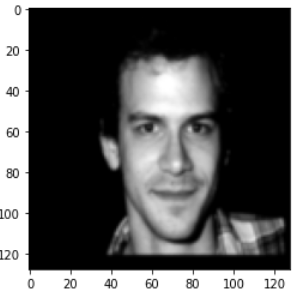
\includegraphics[scale=0.3]{imgs/face_1000.png}
    \caption{Ejemplo de imagen del proyecto \textit{MIT Face Recognition Project}}
    \label{fig:face_1000}
\end{figure}

\subsection{Preprocesamiento de imágenes}
El primer punto es encontrar las dimensiones de cada imagen, las cuales tienen un tamaño de $128\times 128$ pixeles. Posteriormente, hacemos que todas las imágenes se acoplen a estas dimensiones como se muestra a continuación: 

\begin{figure}[H]
    \centering
    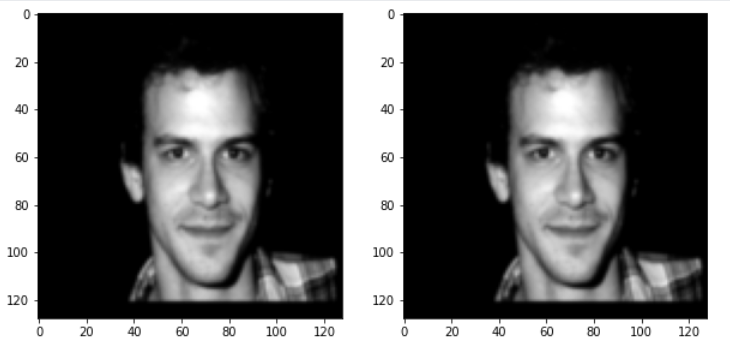
\includegraphics[scale=0.2]{imgs/centered_images.png}
    \caption{Imagen acoplada a una matriz de $128\times 128$}
    \label{fig:faces_centered}
\end{figure}

Una vez que tenemos todas nuestras imágenes con el mismo tamaño, lo que hacemos es encontrar la imagen promedio:

\begin{figure}[H]
    \centering
    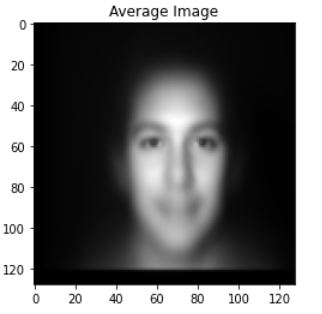
\includegraphics[scale=0.25]{imgs/avg_img.png}
    \caption{Imagen promedio tomada como la media aritmética de cada pixel entre todos los pixeles de todas las imágenes del dataset}
    \label{fig:avg_face}
\end{figure}

La figura \ref{fig:avg_face} se obtiene de realizar el promedio de todas las imágenes del dataset para un pixel en específico. Una vez que tenemos esta figura, lo que hacemos es centrar todas las imágenes mediante la resta de los valores actuales menos los valores de la imagen promedio: 

\begin{figure}[H]
    \centering
    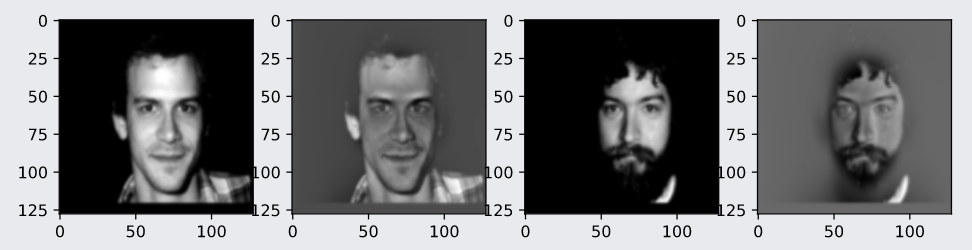
\includegraphics[scale=0.2]{imgs/centered_images_avg.png}
    \caption{Imágenes de caras centradas: resta entre los valores originales y la cara promedio}
    \label{fig:imgs_minus_avg}
\end{figure}

\subsection{PCA}
Para el análisis de componentes principales, empleamos la descomposición por valores singulares para obtener las componentes en orden de importancia. Dichas componentes se almacenan en la matriz $\sigma$ de la ecuación \ref{eq:svd}. 

Al aplicar SVD sobre todo el dataset obtenemos las dimensiones de las matrices de la ecuación \ref{eq:svd}. Los resultados se muestran en la tabla \ref{tab:svd_dimensions}. 

\begin{table}[H]
    \centering
    \begin{tabular}{|c|c|}
         \hline
         Matriz & Dimensiones \\ \hline
         $U$ & $3993 \times 3993$ \\ \hline
         $\Sigma$ & $3993$ \\ \hline
         $V$ & $3993 \times 16384$ \\ \hline
    \end{tabular}
    \caption{Dimensiones de las matrices $U$, $\Sigma$ y $V$}
    \label{tab:svd_dimensions}
\end{table}

Podemos observar que se mantienen las dimensiones de cada matriz de la ecuación \ref{eq:svd_dimesions}. Ahora, para visualizar la variablidad explicada por SVD, podemos recurrir a la figura \ref{fig:svd_graph} en la cual podemos observar que a partir de los primeros $5$ valores singulares, ya no hay variación en los datos. Esto, relacionado con la teoría de SVD, nos indica que podríamos comprimir la información simplemente con $5$ componentes principales y obtener una muy buena aproximación de la información en las caras. 

\begin{figure}[H]
    \centering
    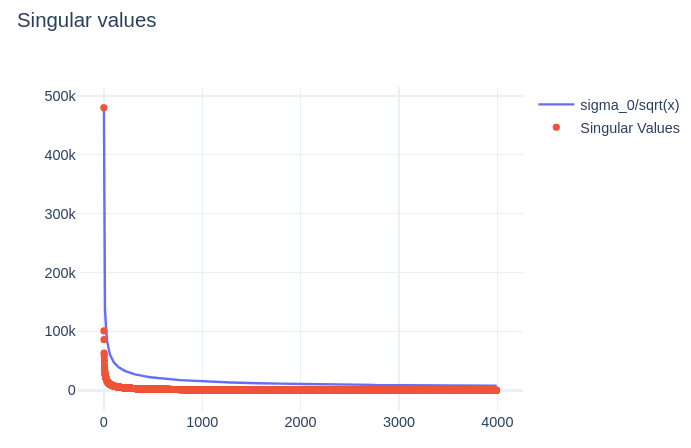
\includegraphics[scale=0.35]{imgs/svd_variance.png}
    \caption{Nivel de variabilidad explicada por cada uno de los $3993$ valores singulares}
    \label{fig:svd_graph}
\end{figure}

En la figura \ref{fig:svd_pc} podemos observar los rasgos explicados por las $5$ componentes principales. A destacar que cada una de las componentes principales explica un rasgo único en las caras. 

\begin{figure}[H]
    \centering
    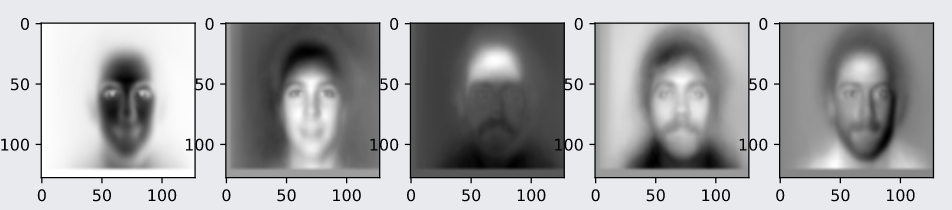
\includegraphics[scale=0.25]{imgs/first_5_pc.png}
    \caption{Rasgos de las caras explicados por las primeras $5$ componentes principales}
    \label{fig:svd_pc}
\end{figure}

Continuando con el tutorial y los ejercicios propuestos en \cite{sandipan}, después se trabajó con la obtención de los \textit{eigenfaces}. Para ello, primero se normalizó y se calcularon los componentes principales de PCA. Esto derivó en que---considerando que se tenían imágenes de tamaño $64 \times 64$ por lo que el tamaño de la matriz era de $4,096$---se redujera el tamaño del vector de componentes principales. Es decir, se proyectaron los valores de los pixeles sobre los $64$ vectores resultantes.

Si observamos la varianza que se va acumulando componente a componente, obtenemos lo siguiente:

\begin{figure}[H]
    \centering
    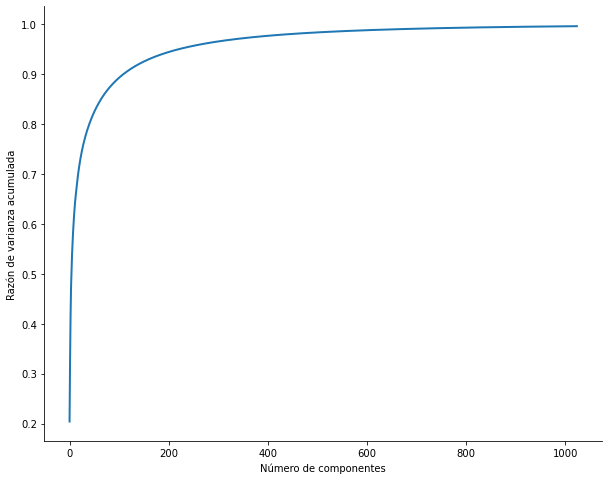
\includegraphics[scale=0.25]{imgs/cum_componentes.png}
    \caption{Acumulado de la varianza por componente calculado.}
    \label{fig:svd_pc}
\end{figure}

En la figura anterior, se muestra claramente que el $90\%$ de las varianzas de las imágenes bajo análisis se encuentran contenidas dentro de las primeras $64$ componentes.

\begin{figure}[H]
    \centering
    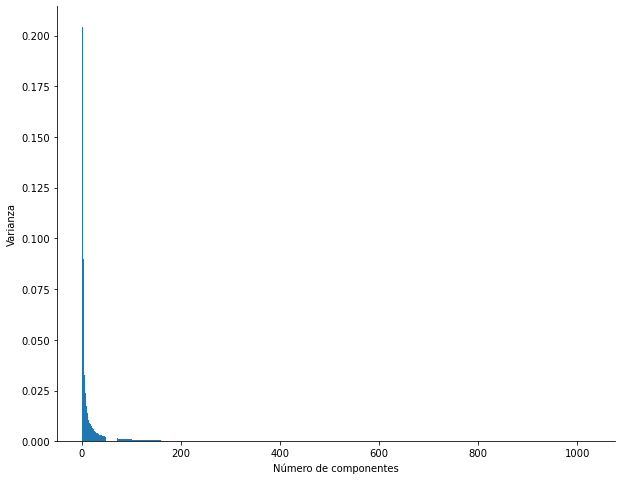
\includegraphics[scale=0.25]{imgs/dist_var.png}
    \caption{Distribución de la varianza dependiente del número de componentes principales considerado. Más del $90\%$ de los elementos se encuentran dentro de los $64$ componentes.}
    \label{fig:svd_pc}
\end{figure}

Ya contando con el procesamiento inicial, se obtuvieron las imágenes promedio y de desviación estándar.

\begin{figure}[H]
    \centering
    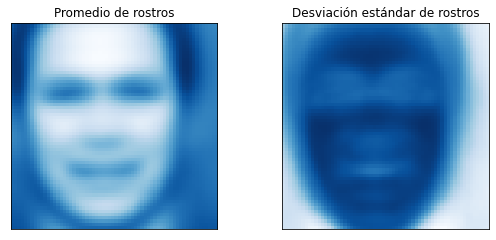
\includegraphics[scale=0.25]{imgs/mean_sd_faces.png}
    \caption{Caras generadas con el promedio y desviación estándar del total de rostros.}
    \label{fig:svd_pc}
\end{figure}

Por lo cual, ya es posible observar las \textit{eigenfaces}, las cuales contienen o describen los elementos más importantes del conjunto original de rostros.

\begin{figure}[H]
    \centering
    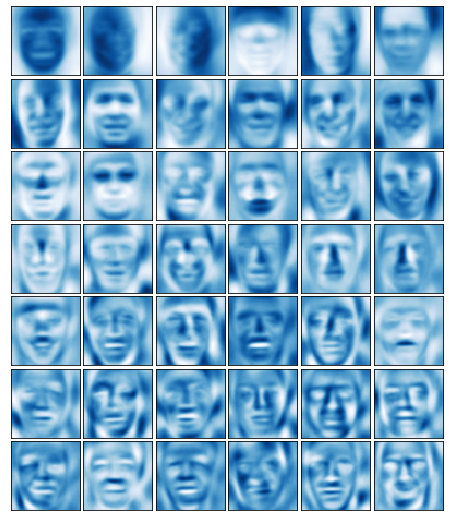
\includegraphics[scale=0.25]{imgs/eigenfaces.png}
    \caption{Se muestran las primeras \textit{eigenfaces}.}
    \label{fig:svd_pc}
\end{figure}

Finalmnete, según lo que se ha incluido en la introducción, en teoría ya es posible reconstruir o generar, a partir de las \textit{eigenfaces}, cualquiera de las imágenes originales en el dataset. Para ello, solo basta con generar una combinación lineal de las $64$ imágenes de referencia basadas en el mismo número de componentes principales. \footnote{Esta función se trabajó a partir del método \textit{inverse\_transform} de scikit\-learn.}

\begin{figure}[H]
    \centering
    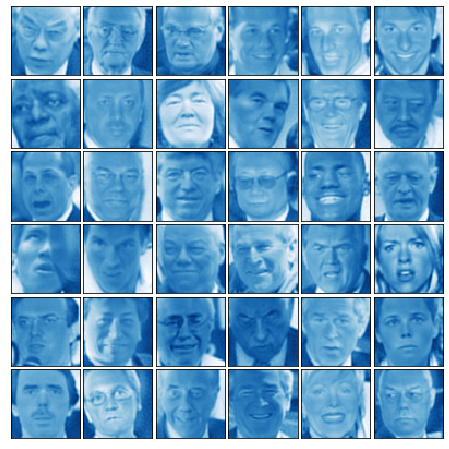
\includegraphics[scale=0.25]{imgs/reconstructed.png}
    \caption{Se muestran imágenes aleatorias regeneradas a partir de los vectores de componentes principales o \textit{eigenfaces}.}
    \label{fig:svd_pc}
\end{figure}

\begin{figure}[H]
    \centering
    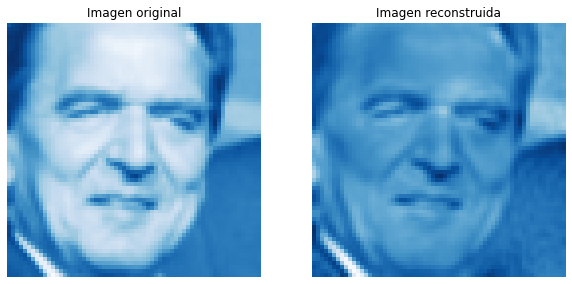
\includegraphics[scale=0.25]{imgs/reconstructed_individual.png}
    \caption{Estudio centrado en la reconstrucción de un rostro en específico a partir de la comparación de la imagen original y la obtenida después de realizar el procesamiento.}
    \label{fig:svd_pc}
\end{figure}

% -------------------------------------------------
% -------------------------------------------------
% -------------------------------------------------
\section{Resultados}

A partir del trabajo realizado, podemos considerar que se ha entendido plenamente el funcionamiento del método de análisis de componentes principales (PCA)---igual que el procesamiento inicial mediante SVD---para generar imágenes que, al ser transformadas linealmente por ciertos parámetros determinados, se pueden combinar para obtener cualquier imagen de una base de datos de fotografías de rostro o cualquier gráfico que se requiera inicial.

La técnica utilizada puede ayudar en la optimización y reducción del espacio para análisis de imágenes, almacenamiento y transmisión de datos gráficos. También, siendo la aplicación más importante de la técnica, este método es fundamental para el reconocimiento de patrones en los rostros y así poder identificar la identidad que se observa en una imagen.

% -------------------------------------------------
% -------------------------------------------------
% -------------------------------------------------
\section{Conclusiones}


% -------------------------------------------------
% -------------------------------------------------
% -------------------------------------------------
\section{Secciones de código relevante}

\subsection{Obtención de la cara promedio}
\begin{lstlisting}[language=python]
def get_avg_image(images): 
    return np.mean(images, axis=0)\end{lstlisting}
    
\subsection{Centrado de imágenes}
\begin{lstlisting}[language=python]
def center_image(image, avg_image):
    return image-avg_image\end{lstlisting}
    
\subsection{SVD}
\begin{lstlisting}[language=Python]
U, Sigma, VT = np.linalg.svd(X, full_matrices=False) \end{lstlisting}

\subsection{Variación de componentes principales}
\begin{lstlisting}[language=python]
x = np.arange(1, Sigma.shape[0])

fig = go.Figure()
fig.add_trace(go.Scatter(
    x=x,
    y=Sigma[0]/np.sqrt(x),
    name='sigma_0/sqrt(x)'
))
fig.add_trace(go.Scatter(
    x=np.arange(Sigma.shape[0]),
    y=Sigma,
    mode='markers', name='Singular Values'
))
fig.update_layout(
    template='plotly_white',
    title=dict(
        text='Singular values'
    ), width=600
)
fig.show() \end{lstlisting}


\subsection{Obtención de las $n$ componentes principales}
\begin{lstlisting}[language=python]
def get_n_principal_components(n, VT):
    images = []
    d = int(np.sqrt(VT[0].shape[0]))
    for i in range(n):
        images.append(VT[i].reshape(d,d))
    return images \end{lstlisting}

% -------------------------------------------------
% -------------------------------------------------
% -------------------------------------------------
\selectlanguage{spanish}
\begin{thebibliography}{}

\bibitem{sandipan} Sandipan D. EigenFaces and A Simple Face Detector with PCA/SVD in Python. sandipanweb, 2021. [Online]. Disponible: \url{https://sandipanweb.wordpress.com/2018/01/06/eigenfaces-and-a-simple-face-detector-with-pca-svd-in-python/}. [Visitado: 06- Aug- 2021]

\bibitem{strang} G. Strang, Introduction to Linear Algebra, Fifth edition. Wellesley: Wellesley-Cambridge Press, 2016. 

\bibitem{szummer} M. Szummer, "Face recognition project", Courses.media.mit.edu, 2002. [Online]. Disponible: https://courses.media.mit.edu/2004fall/mas622j/04.projects/faces/. [Accessed: 08- Aug- 2021]

\end{thebibliography}

\end{document}
